\chapter{Peachpie project}

The Peachpie project\footnote{\href{http://www.peachpie.io/}{peachpie.io/}} aims to create a bridge between PHP and the .NET ecosystem. While its development started in early 2016 it builds upon the foundations of a much older project, Phalanger\footnote{\href{https://github.com/DEVSENSE/Phalanger}{github.com/DEVSENSE/Phalanger}}, first released in 2004 and also originally developed at the Charles University.

While both projects share the same end goal - bring PHP to .NET, their implementation is quite a bit different. Phalanger, due to being first released before even .NET 2.0 shipped, had to implement almost everything itself. Peachpie, on the other hand, relies heavily on components provided by Roslyn infrastructure in compiler and by DLR at runtime.

Also, while Phalanger supports PHP 5.4 as the highest version, Peachpie was built for PHP 7.1 and beyond from the very beginning. The last major difference is that Peachpie, unlike Phalanger, runs not only on full .NET and Mono but also on a multi platform .NET Core framework.

The Peachpie project is, as of early 2017, still in an active pre-version 1.0 development by the open source community. As such its architecture is not yet finalized and might change in the future rendering following chapter inaccurate.


\section{Peachpie architecture}

As already mentioned Peachpie consists of three more or less separate parts. A compiler that takes PHP sources and produces .NET assemblies, runtime library that provides support for various dynamic features of PHP, and a reimplementation of PHP base class library with its most popular extensions. 

Due to the topic of this thesis being an implementation of a compiler feature we will focus mainly on the compiler and only briefly discuss the runtime library. The base class library, while interesting, is completely irrelevant for our work and will be left out.


\section{Peachpie compiler}

The compiler itself is build on the architecture of an open source C\# and Visual Basic compiler platform Roslyn. The compilation is logically divided into four main phases (\autoref{fig3.1:PchpComp}). First a parser takes a PHP source and creates an abstract syntax tree. In Peachpie this step is actually offloaded to a third party open source PHP parser\footnote{\href{https://github.com/DEVSENSE/Parsers}{github.com/DEVSENSE/Parsers}}. Then Peachpie takes over and binds the AST to a semantic representation in form of a control graph, essentially creating an abstract form of the final final program. The binding phase is also responsible for lowering higher level language constructs.

Next, the semantic graph is used for an extensive data-flow analysis with the intention to resolve dynamic types and generally eliminate as much dynamic behaviour as possible. This step is important mainly for performance reasons. Dynamic dispatch and access at runtime inherently brings a performance hit, especially on .NET CLR that, despite being language agnostic, is still tuned mostly for C\# and VB, both of which are statically typed languages.

In the last phase the semantic graph is used to emit the final CIL code and produce a complete .NET assembly. While Peachpie controls the emit of each individual CIL instruction their specific bytecode realization, possible CIL level optimizations, and assembly structure creation is done by Roslyn components \emph{ILBuilder} and \emph{PEBuilder} respectively.

\begin{figure}[h]
	\centering	
	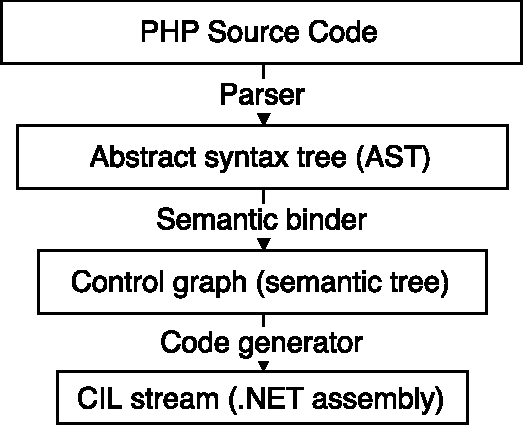
\includegraphics[scale=0.75]{../img/3_1_Peachpie}	
	\caption{Peachpie architecture.}
	\label{fig3.1:PchpComp}
\end{figure}

There is obviously more to the compiler part. It also includes a number of code analyzers to catch common PHP bugs, provides an extensive API surface to support projects such as PHP snippets or Visual Studio Code extension, and much more.

\section{Semantic graph}

Since our approach to implementing generator is based on semantic graph transformation let us explore it a bit more. Unlike AST, which is a structured representation of the source code, the semantic graph corresponds more closely to an abstraction of the final program.

It knows the types of all expressions, has all method calls as well as variable/field accesses resolved and bound to specific semantic symbols, and generally contains all the information needed for future compilation.

\subsection{Statements and expressions}

Before going into specific details about the semantic graph itself let us properly define the difference between expressions and statements first. An expression is a combination of values and operations that produces a new value while potentially also having side effects. 

For example plus is a binary expression that creates a new value from its two children expressions. Method call, if the method returns some value, is an expression as well. Statement, on the other hand, is an operation that only has some side effects and does not carry a value itself. A good example of a statement is goto jump.

This means that in expression trees, a computation abstraction where each node is an operation that takes the values of its children and produces a new value, statements can only be at the top. Since they do not have a value of their own that could be consumed by their potential parent they simply can not have a parent node. 

It is also good to note that while it is simple to transform an expression into a statement from - you simply throw away its value, you can not do it the other way and use a statement in places where expression is expected. 

\subsection{Graph structure}

With that out of the way, semantic graph is fundamentally a forest in which every method declared in the source code or synthesized by the compiler corresponds to its control flow graph. Each graph consist of two types of elements. Edges, representing control flow constructs such as loops, branches, and exception handling constructs, and blocks, simple containers holding standalone semantic statements like method calls, assignments, variable declarations, and so on. 

These individual statements, can have a form of rather complex graphs themselves (\autoref{fig3.3:ExpTree}). They can be arbitrary expression trees with a statement at the top. For example an assignment statement has two expression children, the variable and the one representing the value being assigned. The value expression can also be arbitrary and have children of its own and so on. Semantic expressions and statements are called bound within Peachpie.

\begin{figure}[h]
	\centering	
	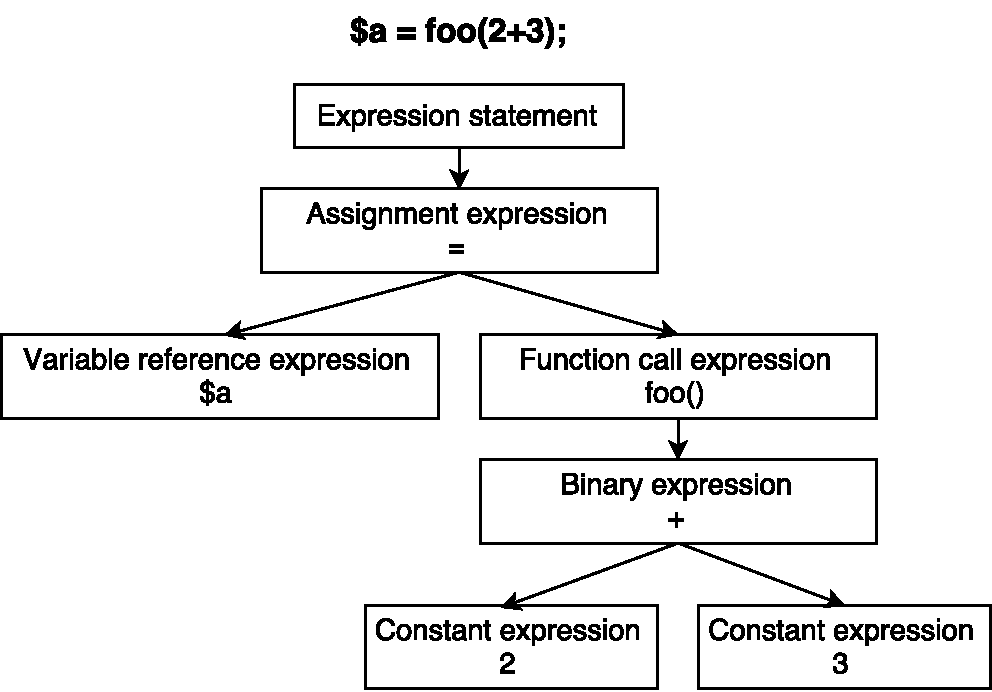
\includegraphics[scale=0.75]{../img/3_3_exprstatements}	
	\caption{Expression tree.}
	\label{fig3.3:ExpTree}
\end{figure}

The control flow edges do not have to be simple and connect only two blocks either. In fact most edges connect multiple blocks and some even have references to individual expressions (\autoref{fig3.3:Edges}). For example a switch edge connects a source block, a switch variable expression, an arbitrary number of case blocks with their case value expressions, and an end block. Other edges are implemented similarly.

\begin{figure}[h]
	\centering	
	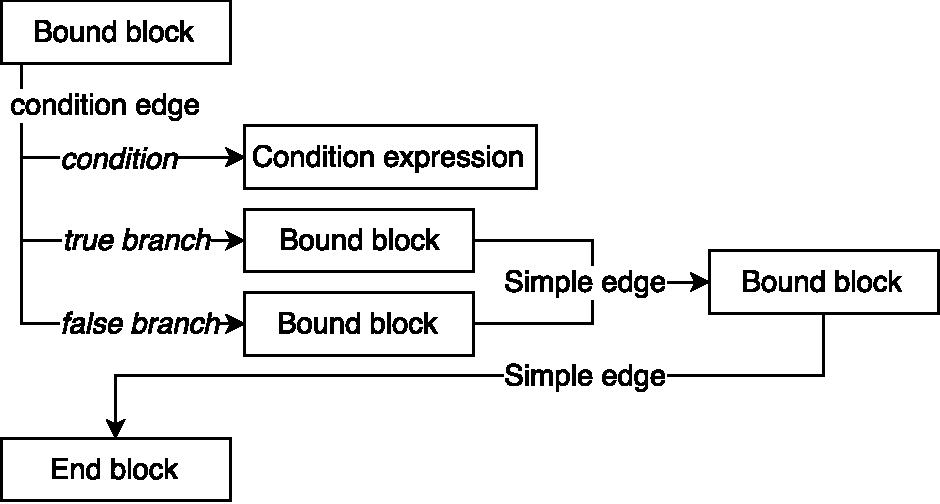
\includegraphics[scale=0.75]{../img/3_3_blocksedges}	
	\caption{Condition edge.}
	\label{fig3.3:Edges}
\end{figure}

The last type of objects to note in regards to semantic graph are symbols. They represent declared objects. These include types, namespaces, methods, fields, variables, and parameters. Read and write accesses to fields, variables, and parameters inside methods are still represented as bound expressions, however. Bound expressions that hold a reference to these symbols and use them as an identifier of the actual place where their value is.

\subsection{Graph creation}

There are two components in Peachpie compiler responsible for the individual method’s control flow graphs creation, \emph{BuilderVisitor} and \emph{SemanticBinder}. \emph{BuilderVisitor} is a higher level component traversing the top level of method’s abstract syntax tree and creating aforementioned control flow edges and bound blocks in the process. 

It uses the \emph{SemanticBinder} to fill these bound blocks with bound statements and to create sporadic bound expressions needed for the edges, e.g. a switch value expression for a switch edge. Specifically it goes through statements and control flow construct in the method’s AST and does two things. It either adds a newly bound statement into the current bound block or, on control flow constructs, creates new bound blocks. When it does that it fills them with statements, connects them to the previous current block, and sets the last of them as the new current block.

The \emph{SemanticBinder} is a component that takes a statement or an expression in form of an abstract syntax tree and creates its semantic representation, either a bound statement or a bound expression, that can be used in the resulting semantic graph. 

It also handles the full complexity of the statements/expressions. When it gets asked by the \emph{BuilderVisitor} to bind an assignment it creates not only the bound assignment statement itself but it binds its children, and their children, and so on as well, returning the full bound subgraph. 

That is the reason why the \emph{BuilderVisitor} goes only through top level statements and does care about individual expressions. With the exception of some within edges, as noted, each expression is part of a larger expression tree under some statement. A statement that gets bind as a whole tree by the \emph{SemanticBinder}. 

\section{CIL emit phase}

In Peachpie the CIL code generation is based solely on the semantic graph. Each of its elements, be it an edge, a statement, or a symbol, has a method, \emph{Generate} or \emph{Emit}, that can create the element’s complete CIL code representation. These methods do not produce the bytecode themselves. Instead the they use a component called \emph{CodeGenerator}, a thin wrapper around Roslyn’s \emph{ILBuilder}.


\subsection{Code generator}
\emph{CodeGenerator} is fundamentally an abstraction of CIL code stream. It can do two things.  Append either individual CIL instructions or their short sequences to the current code stream and realize the stream into actual bytecode. The only higher level service it provides is the ability to change where it should look for certain important items.

One can, for example, set an arbitrary variable as the current this object or specify that local variables should live in some PHP array instead of on the evaluation stack. Appending a load from a local variable then results in the correct CIL sequence being emitted. That means either a load from the locals part of the evaluation stack or, when the place of locals was changed on the current \emph{CodeGenerator}, some \emph{PhpArray}, which itself might need to get loaded from some field first. 

This is used, among other places, when there are indirect variable accesses in a method\footnote{\href{http://php.net/manual/en/language.variables.variable.php}{php.net/manual/en/language.variables.variable.php}}. Because of their indirect and thus dynamic nature it is impossible to resolve and bind them at compilation time. Also there are no CIL instructions to create a new local variable nor to access a variable by its name. Afterall local variables in CIL are just slots in the evaluation stack. Therefore for methods with indirect variables its locals must be moved from the evaluation stack to a \emph{PhpArray} that supports both of these operations.

\subsection{Emit}

The act of emit is very similar to the binding phase. When \emph{Generate} is called on a semantic item it emits CIL representation of not only the item itself but also of all that under it in the semantic graph. A code generation for a method symbol (\autoref{fig3.4:EmitOrder}), for example, causes emit of all of its bound blocks and edges, each of which triggers emit of their bound expressions and statements, effectively ending up with CIL for the whole method’s body being generated. 

As such the emit is effectively a mixture of pre and post-order traversal of the semantic tree. First emit of the current item starts, then its children from left to right get fully emitted, and then it finishes. Due to that and the fact that execution follows the emitted CIL code there is an invariant. Left children represent code that is executed before right children and nodes lower in the tree finish before their parents. 

\begin{figure}[h]
	\centering	
	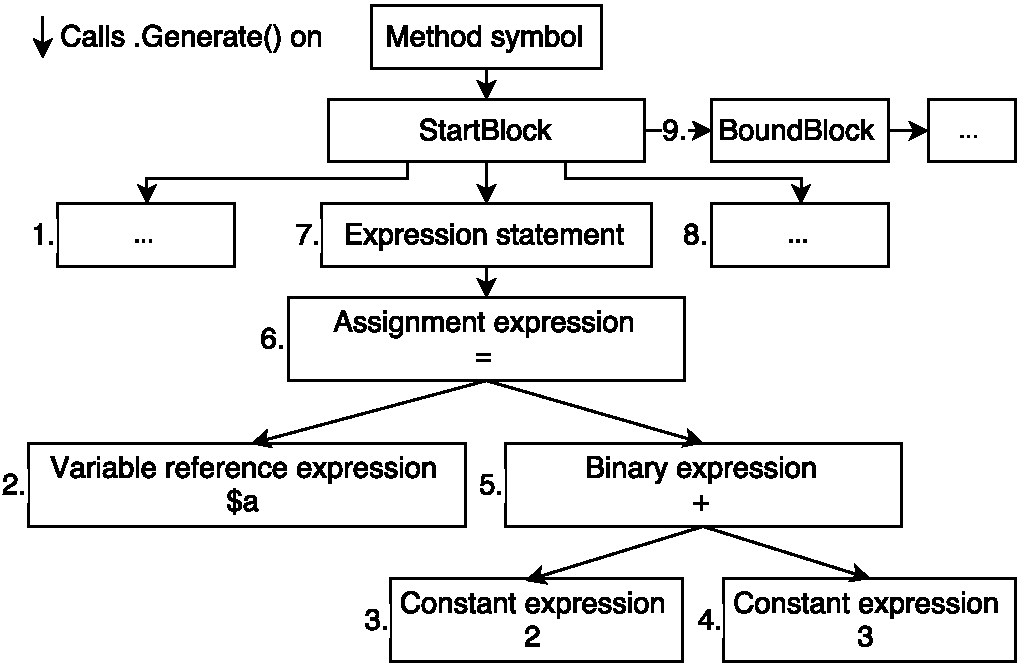
\includegraphics[scale=0.75]{../img/3_4_emitorder}	
	\caption{Emit order of a method.}
	\label{fig3.4:EmitOrder}
\end{figure}

The individual \emph{Generate} or \emph{Emit} methods are completely independent. They only append CIL instructions representing their semantic node to the \emph{CodeGenerator} instance they got passed as a parameter. In case their respective nodes have any children within the semantic graph they also call Generate on them, always passing the \emph{CodeGenerator} instance they themselves got. This ensures that in the end the one \emph{CodeGenerator} instance contains CIL code for all the method’s statements, expressions, and edges.


\subsection{Generate methods’ invariants}

While individual nodes can emit themselves however they want there are two rules that must hold true. The code emitted by a bound expression must load and leave its value on the top the evaluation stack. Other than that it can not leave there anything else nor can it remove something. Their \emph{Generate} methods also have to return a symbol representing the expression’s IL type. 

For bound blocks, statements, and edges the rule is similar with the difference that, since they do not have an inherent value, they can not leave anything on the evaluation stack at all. Their methods do not return anything.

These rules ensure a number of things. First, all expressions are basically interchangeable. An emit of a binary expression does not need to care about the operands’ types. It can simply call \emph{Generate} on them and know the evaluation stack will contain their values, independent on whether they are constant expressions, method calls, or something else.

Also, since neither statements nor edges can leave anything on the evaluation stack and statements can only be at the top level of semantic tree the evaluation stack is guaranteed to be empty in the beginning of each bound statement’s execution. This is important because there are statements, such as return or goto, that transfer execution and therefore need the evaluation stack to be empty.

\section{Peachpie runtime library}

The runtime library consists of a number of important types needed to support the dynamic nature of PHP. Probably the most important one is \emph{PhpValue}, a managed counterpart of Zend Egnine’s \emph{ZVal}\footnote{\href{http://php.net/manual/en/internals2.variables.intro.php}{php.net/manual/en/internals2.variables.intro.php}}. It is a type used everywhere the data-flow analysis can not ensure a more specific type. It is a lightweight struct that can hold a primitive value (number, string, or boolean), \emph{PhpArray} (essentially a hashtable), reference to a proper class instance, or - in case of a reference variable - a link to another \emph{PhpValue}. It also supports all the required type conversions and serves as a true representation for an arbitrary PHP value.

Another core type present in the runtime library is \emph{Context}. As hinted by its name it holds the context of the current execution. Be it defined global methods, variables, and constants, the value of static fields and much more. It is a rather special type because it gets silently passed to every PHP method as their first argument throughout the whole execution.

When a library originally written in PHP is used from another .NET language the context has to be explicitly created and passed into it as part of an invocation. If the original PHP app is used on its own the context gets created automatically in the beginning before any user code is run.

Other than that the runtime library also contains function call and variable access resolution logic needed to support dynamic behaviors at runtime, variety of types needed for certain PHP features such as base class for lambdas, and full reflection support. 
